\documentclass[dvisvgm]{standalone}
\usepackage{tikz}

\usetikzlibrary {arrows.meta,automata,positioning}
\begin{document}
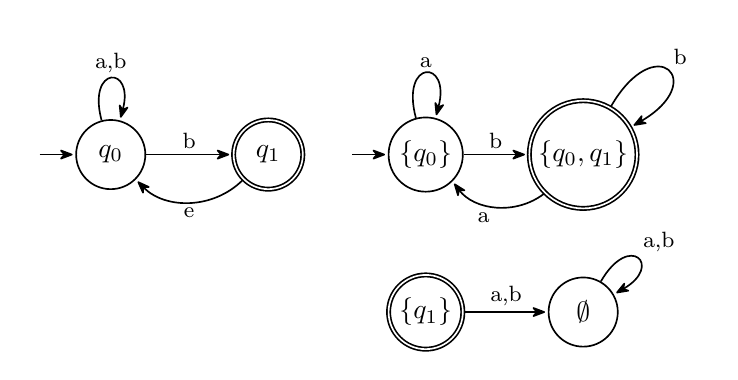
\begin{tikzpicture}[->,>={Stealth[round]},shorten >=1pt,%
    auto,node distance=2cm,on grid,semithick,
    inner sep=2pt,bend angle=45,initial text=]
    \node[initial,state]    (q_0)                   {$q_0$};
    \node[state,accepting]  (q_1) [right=of q_0]    {$q_1$};
    \node[initial,state]    (p_0) [right=of q_1]    {$\{q_0\}$};
    \node[state,accepting]  (p_1) [right=of p_0]    {$\{q_0,q_1\}$};
    \node[state,accepting]  (p_2) [below=of p_0]    {$\{q_1\}$};
    \node[state]            (p_3) [right=of p_2]    {$\emptyset$};
    
    \path [every node/.style={font=\footnotesize}]
        (q_0) edge [loop above]         node {a,b} (q_0)
              edge                      node {b}   (q_1)
        (q_1) edge [bend left]          node {e}   (q_0)
        (p_0) edge [loop above]         node {a}   (p_0)
              edge                      node {b}   (p_1)
        (p_1) edge [bend left]          node {a}   (p_0)
              edge [in=30,out=60,loop]  node {b}   (p_1)
        (p_2) edge                      node {a,b} (p_3)
        (p_3) edge [in=30,out=60,loop]  node {a,b} (p_3);
\end{tikzpicture}
\end{document}
